% ============================================================
%  Capítulo 5 — Representação Intermediária Cross-Engine
% ============================================================
\chapter{REPRESENTAÇÃO INTERMEDIÁRIA CROSS-ENGINE}
\label{cap:ir}

\section{Motivação: vocabulários disjuntos entre V8 e SpiderMonkey}
\label{sec:ir-motivacao}

A detecção de fingerprinting baseada em bytecodes pressupõe que o
classificador opere sobre um espaço de features compartilhado entre os motores que
se deseja suportar. Essa condição não é satisfeita por nenhum conjunto de opcodes
nativo: os conjuntos de instrução do V8 (Ignition) e do SpiderMonkey são definidos
independentemente por suas equipes de desenvolvimento e não possuem nomes em comum.

Além da diferença nominal, os dois motores adotam arquiteturas de máquina virtual
distintas. O V8 utiliza uma \textbf{máquina de registradores com acumulador
implícito}: cada instrução opera sobre o acumulador e, opcionalmente, sobre
registradores explicitamente nomeados. O SpiderMonkey utiliza uma \textbf{máquina
de pilha}: operandos são empilhados explicitamente antes de cada instrução e o
resultado é depositado no topo da pilha. Uma operação aritmética que o V8 codifica
em uma única instrução, por exemplo, \texttt{Add r1} (soma o registrador
\texttt{r1} ao acumulador), requer três instruções no SpiderMonkey:
\texttt{GetLocal 0; GetLocal 1; Add}. Isso implica que a mesma função JavaScript
produz sequências de bytecodes de comprimentos diferentes e com tokens distintos
nos dois motores.

A Tabela~\ref{tab:opcodes-divergencia} ilustra a divergência para um trecho
representativo de código de fingerprinting, leitura de
\texttt{navigator.hardwareConcurrency}:

\begin{table}[htb]
\centering
\caption{Opcodes para \texttt{let x = navigator.hardwareConcurrency}}
\label{tab:opcodes-divergencia}
\begin{tabular}{lll}
\toprule
\textbf{Passo semântico} & \textbf{V8 (Ignition)} & \textbf{SpiderMonkey} \\
\midrule
Carregar \texttt{navigator}           & \texttt{LdaGlobal}       & \texttt{GetGName} \\
Ler \texttt{.hardwareConcurrency}     & \texttt{GetNamedProperty} & \texttt{GetProp} \\
Armazenar em variável local           & \texttt{Star0}            & \texttt{SetLocal} \\
\bottomrule
\end{tabular}
\fonte{Elaborada pelo autor.}
\end{table}

Treinar um classificador TF-IDF diretamente sobre bytecodes brutos de um motor e
aplicá-lo ao outro é equivalente a usar vocabulários completamente disjuntos:
nenhum feature do modelo de origem existe no espaço de features do destino. Os
experimentos de transferência zero-shot (Capítulo~\ref{cap:experimentos}) confirmam
empiricamente essa intuição, com F1 entre 0,149 e 0,180.

A solução proposta neste trabalho é uma \textbf{representação intermediária
cross-engine (RI)}: um vocabulário fixo de tokens abstratos que substituem os
opcodes nativos de ambos os motores, preservando as distinções semânticas relevantes
para a tarefa de classificação de fingerprinting. O mesmo trecho acima,
traduzido para a RI, torna-se \texttt{LOAD\_GLOBAL, GET\_NAMED\_PROP, STORE\_LOCAL}
em ambos os motores.

%, , , , , , , , , , , , , , , , , , , --
\section{Metodologia dos micro-scripts}
\label{sec:micro}

\subsection{Motivação para a abordagem empírica}
\label{sub:micro-motivacao}

A correspondência entre opcodes dos dois motores não pode ser derivada
automaticamente a partir de suas especificações: não existe documentação formal que
mapeie instruções V8 para instruções SpiderMonkey. A única fonte de verdade é a
observação empírica: executar o mesmo código JavaScript nos dois motores
instrumentados e comparar as sequências de bytecodes produzidas.

Para que o mapeamento seja exaustivo e auditável, é necessário que os scripts de
teste cubram sistematicamente as construções JavaScript relevantes para
fingerprinting, uma por vez, de forma que a correspondência entre opcodes
possa ser estabelecida por inspeção direta da saída.

\subsection{Conjunto de micro-scripts}
\label{sub:micro-conjunto}

Foram elaborados 27 micro-scripts JavaScript, cada um
exercitando uma construção isolada. A Tabela~\ref{tab:micro} lista os scripts e as
construções cobertas.


\begin{longtable}{l p{0.55\linewidth}}
\caption{Micro-scripts e construções JavaScript cobertas}
\label{tab:micro} \\
\toprule
\textbf{Script} & \textbf{Construção} \\
\midrule
\endfirsthead
\toprule
\textbf{Script} & \textbf{Construção} \\
\midrule
\endhead
\bottomrule
\endlastfoot
\texttt{01\_literals.js}       & Literais numéricos, booleanos, \texttt{null}, \texttt{undefined} \\
\texttt{02\_local\_vars.js}    & Leitura e escrita de variáveis locais \\
\texttt{03\_global\_vars.js}   & Leitura e escrita de variáveis globais \\
\texttt{04\_closure\_vars.js}  & Leitura e escrita de variáveis de closure (upvalues) \\
\texttt{05\_property\_read.js} & Leitura de propriedade nomeada (\texttt{obj.prop}) \\
\texttt{06\_property\_write.js}& Escrita de propriedade nomeada (\texttt{obj.prop = v}) \\
\texttt{07\_keyed\_read.js}    & Leitura de propriedade indexada (\texttt{obj[key]}) \\
\texttt{08\_keyed\_write.js}   & Escrita de propriedade indexada (\texttt{obj[key] = v}) \\
\texttt{09\_arithmetic.js}     & Operações aritméticas (\texttt{+}, \texttt{-}, \texttt{*}, \texttt{/}, \texttt{\%}, \texttt{**}) \\
\texttt{10\_bitwise.js}        & Operações bitwise (\texttt{|}, \texttt{\&}, \texttt{\textasciicircum}, \texttt{<<}, \texttt{>>}, \texttt{>>>}) \\
\texttt{11\_unary.js}          & Operadores unários (\texttt{-}, \texttt{\textasciitilde}, \texttt{!}, \texttt{++}, \texttt{--}) \\
\texttt{12\_comparisons.js}    & Comparações (\texttt{==}, \texttt{===}, \texttt{<}, \texttt{>}, \texttt{<=}, \texttt{>=}) \\
\texttt{13\_typeof.js}         & Operador \texttt{typeof} \\
\texttt{14\_conditional.js}    & Desvios condicionais (\texttt{if}/\texttt{else}, operador ternário) \\
\texttt{15\_loops.js}          & Laços (\texttt{for}, \texttt{while}, \texttt{do...while}) \\
\texttt{16\_logical.js}        & Operadores lógicos de curto-circuito (\texttt{\&\&}, \texttt{||}, \texttt{??}) \\
\texttt{17\_method\_call.js}   & Chamada de método (\texttt{obj.method(args)}) \\
\texttt{18\_function\_call.js} & Chamada de função pura (\texttt{func(args)}) \\
\texttt{19\_constructor.js}    & Construção de objeto (\texttt{new Class(args)}) \\
\texttt{20\_return.js}         & Instrução \texttt{return} \\
\texttt{21\_closure\_create.js}& Criação de closure \\
\texttt{22\_object\_literal.js}& Literal de objeto (\texttt{\{ k: v \}}) \\
\texttt{23\_array\_literal.js} & Literal de array (\texttt{[a, b, c]}) \\
\texttt{24\_try\_catch.js}     & Bloco \texttt{try}/\texttt{catch}/\texttt{throw} \\
\texttt{25\_type\_coercion.js} & Coerções de tipo (\texttt{Number()}, \texttt{String()}, \texttt{Boolean()}) \\
\texttt{26\_instanceof.js}     & Operador \texttt{instanceof} \\
\texttt{27\_string\_concat.js} & Concatenação de strings \\
\end{longtable}

As construções escolhidas cobrem intencionalmente os padrões observados no topo da
lista de importância de features (Capítulo~\ref{cap:experimentos}): acesso a
propriedades (scripts 05--08), chamadas de método e função (17, 18), variáveis de
closure (04, 21) e desvios condicionais com \texttt{try/catch} (14, 24).

\subsection{Execução pareada e alinhamento}
\label{sub:micro-exec}

Cada micro-script é executado nos dois navegadores instrumentados por um script
de automação. Para cada execução, captura-se a sequência de bytecodes emitida
pelo motor para a função principal do micro-script e salva-se o resultado com
as sequências de cada motor.

O alinhamento é feito em duas etapas:

\begin{enumerate}
\item \textbf{Alinhamento manual.} Para cada par
  \texttt{(v8\_bytecodes, sm\_bytecodes)}, os opcodes são inspecionados
  visualmente e agrupados por correspondência semântica. A diferença de
  arquitetura (registrador vs. pilha) exige mapeamentos de cardinalidade
  N:1 ou 1:N em alguns casos, por exemplo, um único \texttt{Add} do V8 pode
  corresponder a \texttt{GetLocal; GetLocal; Add} do SpiderMonkey, mas todos os
  três são mapeados para o mesmo token de RI \texttt{BINARY\_ADD}.

\item \textbf{Validação estatística.} O validador aplica o mapeamento estático
  ao corpus de micro-scripts e calcula a cobertura dos opcodes observados.
  Mapeamentos que deixam opcodes frequentes sem correspondência são revisados
  até que a cobertura do corpus de micro-scripts atinja 100\%.
\end{enumerate}

A Figura~\ref{fig:ir-metodologia} sintetiza essa metodologia.

\begin{figure}[htb]
\centering
\caption{Metodologia de construção da representação intermediária cross-engine}
\label{fig:ir-metodologia}
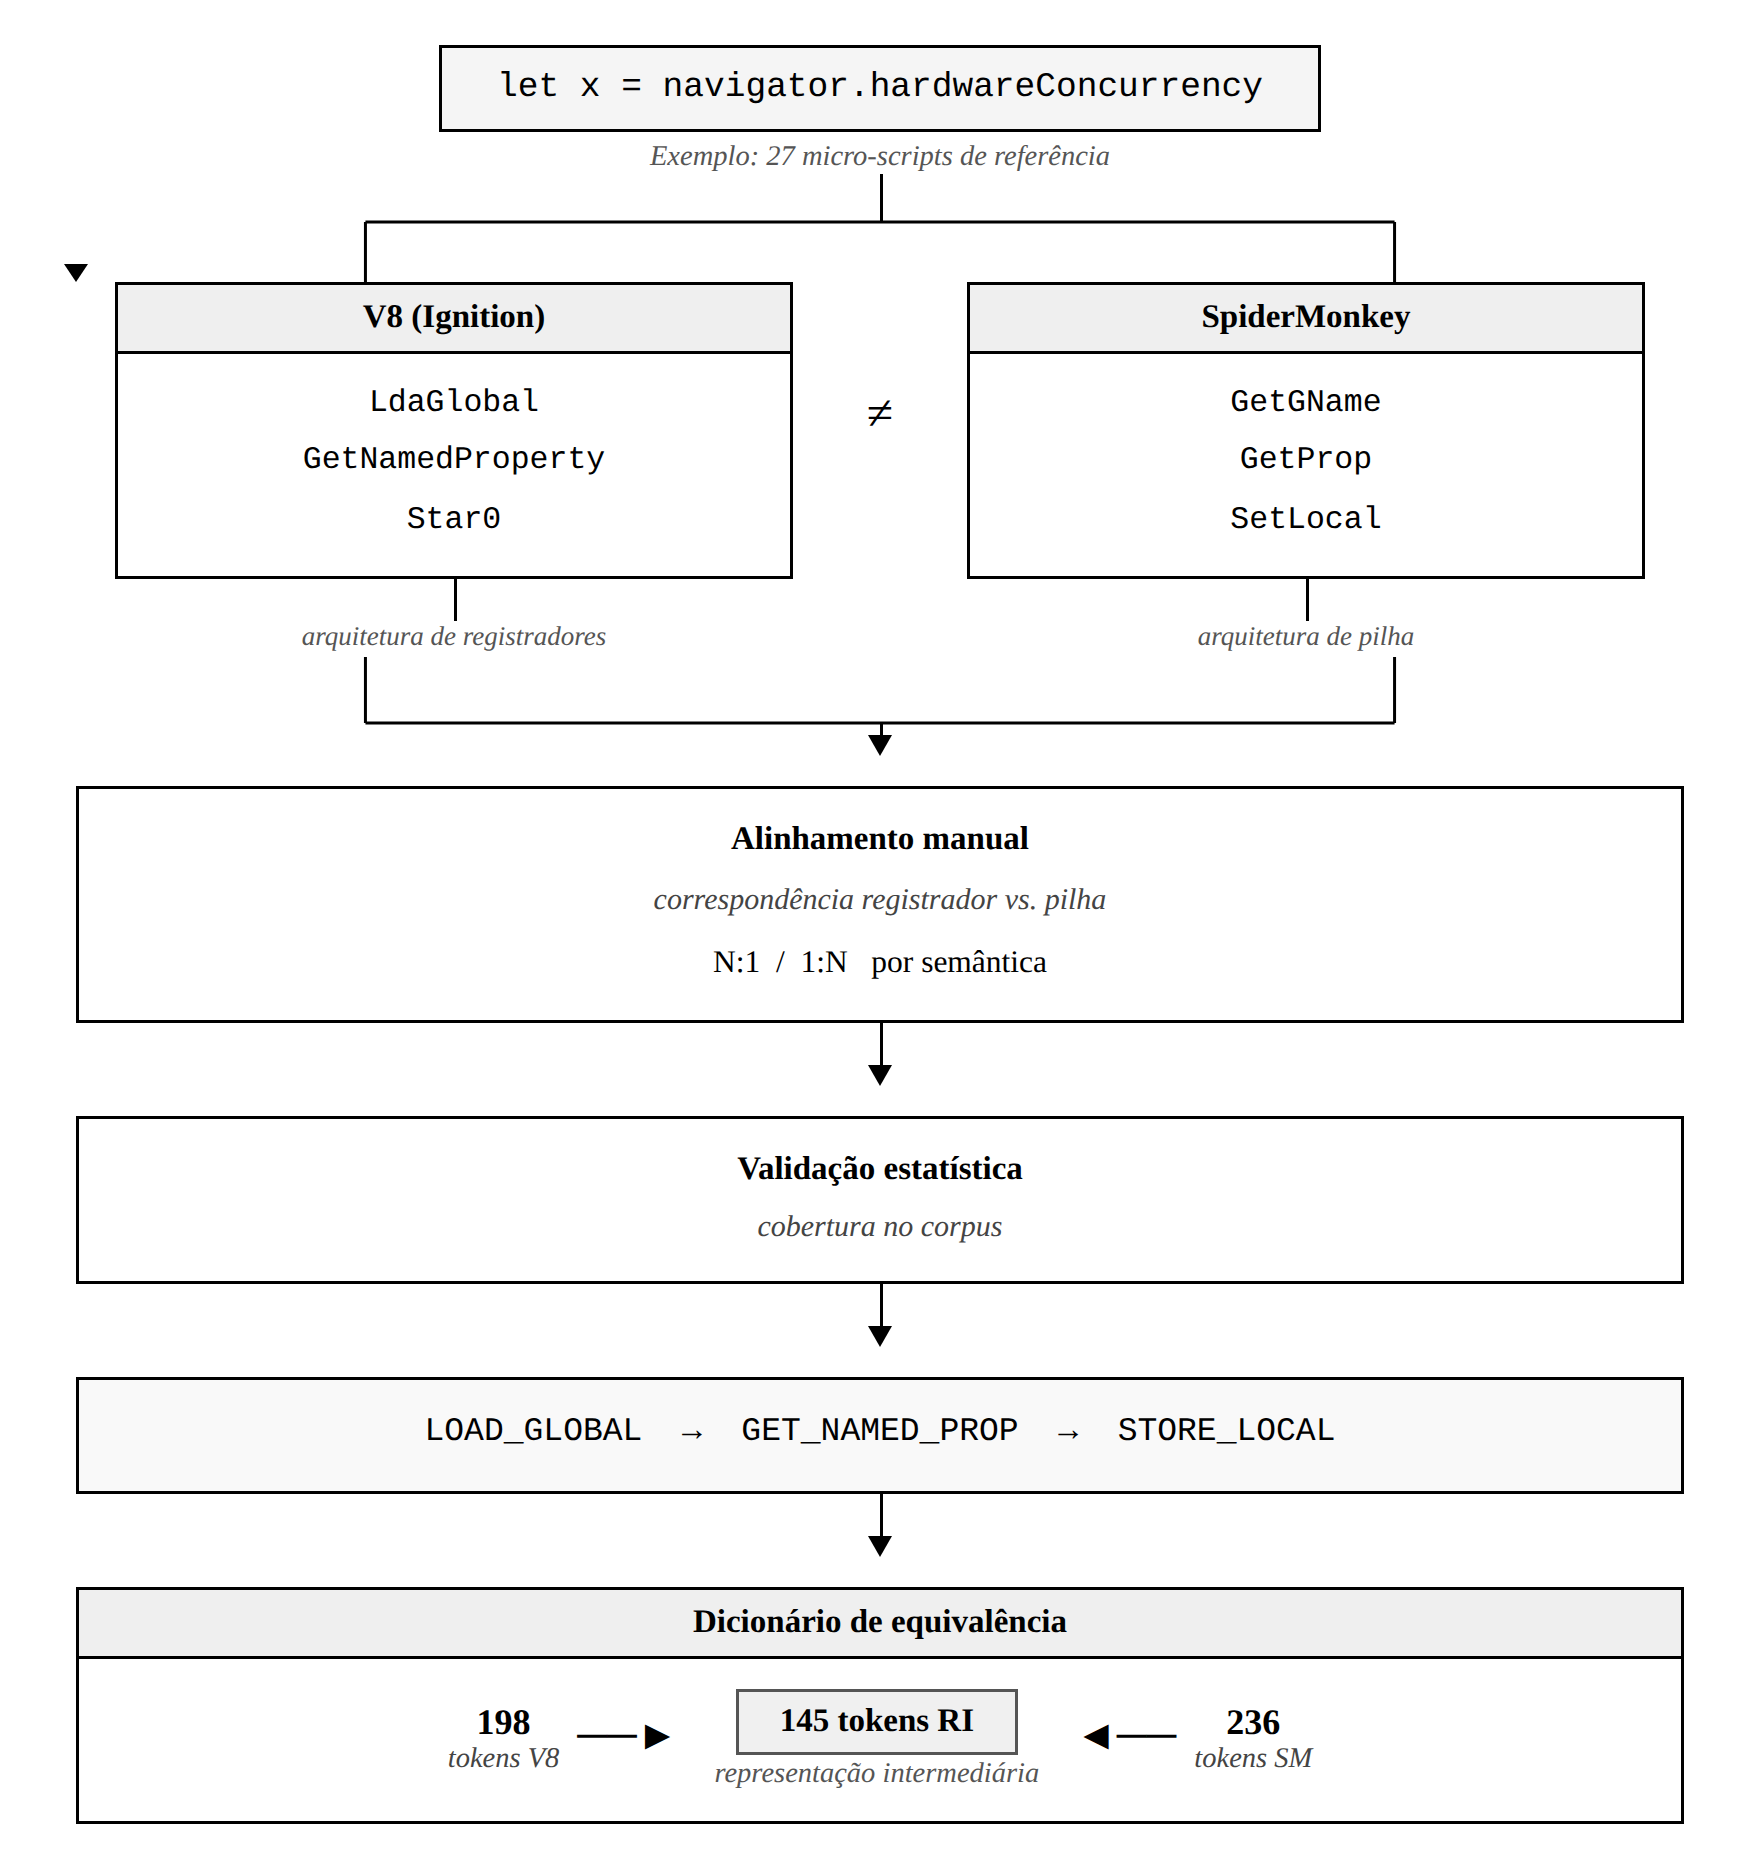
\includegraphics[width=0.92\linewidth]{fig_ir_methodology}

\fonte{Elaborada pelo autor.}
\end{figure}

%, , , , , , , , , , , , , , , , , , , --
\section{Dicionário de equivalência}
\label{sec:dict}

\subsection{Estrutura e dimensões}
\label{sub:dict-estrutura}

O dicionário de equivalência contém dois mapeamentos planos: \texttt{v8\_to\_ir}
(198 entradas) e \texttt{sm\_to\_ir}
(236 entradas), ambos mapeando para o mesmo conjunto de 145 tokens de RI. O número
maior de entradas no lado SpiderMonkey reflete a granularidade mais alta do
conjunto de instrução de pilha: construções que o V8 codifica em poucos opcodes
correspondem a múltiplos opcodes especializados no SpiderMonkey sob o mesmo token de RI.
Por exemplo, o token \texttt{LOAD\_INT} cobre apenas \texttt{LdaZero} e \texttt{LdaSmi}
no V8, mas seis variantes no SpiderMonkey (\texttt{Zero}, \texttt{One}, \texttt{Int8},
\texttt{Int32}, \texttt{Uint16}, \texttt{Uint24}).

A Tabela~\ref{tab:dict-exemplos} apresenta exemplos representativos do dicionário
para as categorias de maior importância discriminativa.

\begin{table}[htb]
\centering
\caption{Exemplos de mapeamentos por categoria no dicionário de equivalência}
\label{tab:dict-exemplos}
\begin{tabularx}{\linewidth}{l>{\raggedright\arraybackslash}X>{\raggedright\arraybackslash}X}
\toprule
\textbf{Token de RI} & \textbf{Opcodes V8 mapeados} & \textbf{Opcodes SM mapeados} \\
\midrule
\texttt{GET\_KEYED\_PROP}   & \texttt{GetKeyedProperty}, \texttt{GetEnumeratedKeyedProperty} & \texttt{GetElem} \\
\texttt{GET\_NAMED\_PROP}   & \texttt{GetNamedProperty}, \texttt{GetNamedPropertyFromSuper} & \texttt{GetProp} \\
\texttt{LOAD\_CLOSURE\_VAR} & \texttt{LdaContextSlot}, \ldots\ (13 variantes) & \texttt{GetAliasedVar} \\
\texttt{CALL\_FUNC}         & --- & \texttt{Call}, \texttt{CallIgnoresRv}, \ldots \\
\texttt{CALL\_FUNC\_N}      & \texttt{CallUndefinedReceiver}, \texttt{CallAnyReceiver}, \texttt{CallWithSpread} & --- \\
\texttt{CALL\_METHOD\_N}    & \texttt{CallProperty} & --- \\
\texttt{BINARY\_ADD}        & \texttt{Add}, \texttt{AddSmi} & \texttt{Add} \\
\texttt{STORE\_LOCAL}       & \texttt{Star}, \texttt{Star0}--\texttt{Star15}, \texttt{Mov} & \texttt{SetLocal} \\
\texttt{TRY\_START}         & ---                                                     & \texttt{Try} \\
\bottomrule
\end{tabularx}
\fonte{Elaborada pelo autor.}
\end{table}

O V8 possui variantes \texttt{*Smi} para operações aritméticas e bit a bit que são
caminhos rápidos especializados para inteiros pequenos (small integers).
Essas variantes não têm equivalente direto no SpiderMonkey e são mapeadas para o
mesmo token de RI que a instrução genérica correspondente.

\subsection{Cobertura no corpus real}
\label{sub:dict-cobertura}

A cobertura foi medida sobre o corpus completo de 68 milhões de funções,
que contém 4,41 bilhões de tokens de bytecodes nativos distribuídos entre os
dois motores. A cobertura de 99,82\% é calculada sobre o corpus misto; o valor
é reportado por motor na tabela abaixo como a fração dos tokens daquele motor
que possui mapeamento no dicionário.

\begin{table}[htb]
\centering
\caption{Cobertura do dicionário de equivalência no corpus real}
\label{tab:cobertura}
\begin{tabular}{lrr}
\toprule
\textbf{Métrica} & \textbf{V8} & \textbf{SpiderMonkey} \\
\midrule
Mapeamentos no dicionário           & 198    & 236    \\
Cobertura de tokens (\% do total)   & 99,82\% & 99,82\% \\
Tokens não mapeados $\to$ \texttt{<UNK>} & $\approx$0,18\% & $\approx$0,18\% \\
\bottomrule
\end{tabular}
\fonte{Elaborada pelo autor.}
\end{table}

Os tokens não mapeados ($\approx$0,18\%) correspondem a opcodes específicos de
versões recentes do V8 e do SpiderMonkey não cobertos pelo conjunto de 27
micro-scripts, como variantes de instruções de feedback de tipo e opcodes
introduzidos após a construção do dicionário. As instruções de gerador/assíncrono e
de módulo ES têm mapeamentos explícitos no dicionário (ver Apêndice~\ref{ap:ir-dict},
seção \textit{Generators, async e miscelânea}) e não contribuem para o
\texttt{<UNK>}. Dois tokens de RI nunca aparecem no corpus real, \texttt{SCOPE\_INIT} e \texttt{WIDE\_PREFIX};
os 143 restantes reduzem-se a \textbf{136 tokens ativos} após filtragem por frequência
mínima (\texttt{min\_df}) nos conjuntos de treinamento amostrados.

%, , , , , , , , , , , , , , , , , , , --
\section{Pipeline de tradução do dataset}
\label{sec:traducao}

O pipeline de tradução lê o dataset limpo um grupo de linhas (row group) por
vez (o arquivo possui 401 grupos com $\approx$170 mil linhas cada) e
aplica a tradução token a token, produzindo o dataset traduzido.

Para cada função, o campo \texttt{browser} determina qual mapeamento usar
(\texttt{sm\_to\_ir} para Firefox ou \texttt{v8\_to\_ir} para Chromium). Os
bytecodes separados por vírgula são traduzidos token a token; tokens ausentes no
dicionário recebem o símbolo especial \texttt{<UNK>}. O delimitador muda de
vírgula para espaço na sequência de RI, alinhando-se ao formato esperado pelo
TF-IDF e pelo FastText. A coluna de bytecodes é substituída pela sequência de
tokens de RI; todas as demais colunas são preservadas.

O processamento em streaming mantém o pico de memória em $\approx$4~GB
(dominado pelo grupo de linhas corrente mais os buffers de escrita PyArrow),
viabilizando a execução em máquinas com 16~GB de RAM sem armazenamento temporário
em disco.

%, , , , , , , , , , , , , , , , , , , --
\section{Embeddings FastText}
\label{sec:embeddings}

\subsection{Construção do corpus de treinamento}
\label{sub:corpus}

O corpus de treinamento é gerado iterando todas as 68 milhões de sequências
de tokens de RI do dataset traduzido. Duas situações de borda são tratadas:

\textbf{Sequências muito curtas.} Funções com menos de 2 tokens de RI (811
stubs com apenas \texttt{RETURN}) são descartadas: não possuem janela de
contexto válida para o algoritmo Skip-gram e produziriam gradientes inválidos.

\textbf{Sequências muito longas.} Funções com mais de 512 tokens são divididas em
fragmentos não sobrepostos de 512 tokens cada, sem descarte de tokens. A divisão é
semanticamente equivalente à sequência completa para o Skip-gram, que opera sobre
janelas de contexto locais de $\pm$5 posições, a co-ocorrência entre tokens
distantes não é capturada de qualquer forma. A alternativa de truncar em 512
descartaria silenciosamente tokens de fingerprinting que aparecem no final
de funções longas.

\subsection{Decisões críticas de treinamento}
\label{sub:fasttext-decisoes}

\textbf{Algoritmo: Skip-gram, não CBOW.} O CBOW (Word2Vec) foi treinado e
descartado. Com um vocabulário fechado de 145 tokens, o amostrador negativo do CBOW
escolhe com alta frequência o próprio token positivo como amostra negativa, gerando
gradientes contraditórios. O resultado foi colapso de vetores: 5 vetores com
NaN/Inf, 28 vetores com norma zero, e coerência semântica de categoria $-0{,}010$
(pior que aleatório). O Skip-gram inverte o problema de predição, prevê o
contexto a partir da palavra central, e produz gradientes bem definidos mesmo
com vocabulário pequeno.

\textbf{Subsampling desativado ($t = 0{,}0$).} O parâmetro $t$ controla a taxa de
descarte de tokens de alta frequência durante o treinamento. O valor padrão
$t = 1 \times 10^{-4}$ descarta tokens cujas frequências relativas excedem o
limiar. Com apenas 145 tipos no vocabulário, todos os tokens qualificam-se como
``alta frequência'' sob esse critério, e virtualmente todo o sinal de treinamento é
eliminado nas primeiras iterações. Definir $t = 0{,}0$ desativa o subsampling
completamente, que é o comportamento correto para um vocabulário fechado desta
magnitude.

\textbf{\texttt{minCount = 1}.} Para garantir que todos os 145 tokens de RI
recebam vetores mesmo que apareçam raramente no corpus, o limiar mínimo de
frequência é fixado em~1.

\textbf{Hiperparâmetros de treinamento:}

\begin{table}[htb]
\centering
\caption{Hiperparâmetros do modelo FastText Skip-gram}
\label{tab:fasttext-hp}
\begin{tabular}{ll}
\toprule
\textbf{Parâmetro} & \textbf{Valor} \\
\midrule
Algoritmo            & Skip-gram \\
Dimensão             & 128 \\
Épocas               & 5 \\
Janela de contexto   & 5 \\
\texttt{minCount}    & 1 \\
Subsampling $t$      & 0,0 \\
Threads       & 4 \\
Chunk size    & 512 tokens \\
\bottomrule
\end{tabular}

\fonte{Elaborada pelo autor.}
\end{table}

\subsection{Avaliação dos embeddings}
\label{sub:fasttext-eval}

\textbf{Saúde dos vetores.} O modelo FastText resultante não apresenta vetores
degenerados: 0 vetores NaN/Inf, 0 vetores de norma zero, norma média de 0,0061, e
similaridade de cosseno média entre pares de 0,017, indicando que o espaço
vetorial está bem distribuído e não colapsado.

\textbf{Coerência semântica de categoria.} O avaliador de embeddings computa, para cada categoria de opcode, a
similaridade de cosseno média intra-categoria (pares de tokens na mesma
categoria) e inter-categoria (pares entre categorias distintas). O
gap positivo confirma que tokens semanticamente relacionados estão mais
próximos entre si do que de tokens de outras categorias.

\begin{table}[htb]
\centering
\caption{Coerência por categoria de token de RI (FastText Skip-gram)}
\label{tab:coerencia}
\begin{tabular}{lrrr}
\toprule
\textbf{Categoria} & \textbf{Intra} & \textbf{Inter} & \textbf{Gap} \\
\midrule
\texttt{PROP\_GET} & 0,505 &  0,047 & \textbf{+0,458} \\
\texttt{BINARY}    & 0,478 & $-0{,}004$ & \textbf{+0,482} \\
\texttt{CREATE}    & 0,436 &  0,005 & \textbf{+0,431} \\
\texttt{CALL}      & 0,355 &  0,005 & \textbf{+0,350} \\
\texttt{LOAD}      & 0,328 &  0,004 & \textbf{+0,324} \\
\texttt{BITWISE}   & 0,331 &  0,010 & \textbf{+0,321} \\
\texttt{PROP\_SET} & 0,286 &  0,033 & \textbf{+0,253} \\
\texttt{STORE}     & 0,251 &  0,007 & \textbf{+0,244} \\
\texttt{CMP}       & 0,201 & $-0{,}003$ & \textbf{+0,204} \\
\texttt{UNARY}     & 0,142 &  0,015 & \textbf{+0,127} \\
\texttt{JMP}       & 0,054 &  0,001 & \textbf{+0,053} \\
\texttt{COERCE}    & 0,052 &  0,004 & \textbf{+0,048} \\
\texttt{CONTROL}   & $-0{,}006$ & $-0{,}010$ & \textbf{+0,004} \\
\midrule
\textbf{GERAL}     & \textbf{0,245} & \textbf{0,008} & \textbf{+0,237} \\
\bottomrule
\end{tabular}

\fonte{Elaborada pelo autor.}
\end{table}

As categorias \texttt{PROP\_GET} e \texttt{BINARY} apresentam os maiores
gaps, refletindo a alta co-ocorrência contextual entre tokens de acesso a
propriedades (típicos de código de fingerprinting) e entre operadores
aritméticos. A categoria \texttt{CONTROL}, que agrupa \texttt{RETURN},
\texttt{POP}, \texttt{THROW} e \texttt{SWAP}, apresenta gap próximo de
zero por ser semanticamente heterogênea: esses tokens não compartilham contexto de
co-ocorrência, e o modelo corretamente os representa com vetores dissimilares.

\textbf{Independência de motor.} O modelo foi treinado sobre o corpus misto
(Firefox + Chromium) sem rótulo de motor. Qualquer estrutura de agrupamento no
espaço vetorial é portanto intrinsecamente cross-engine: quando \texttt{BINARY\_ADD}
aparece em uma sequência SpiderMonkey e em uma sequência V8, ambas as ocorrências
contribuem para o mesmo vetor. O gap de coerência geral de +0,237 confirma
que o modelo aprendeu estrutura semântica a partir desse sinal combinado.
